%%%%%%%%%%%%%%%%%%%%%%%%%%%%%%%%%%%%%%%%%%%%%%%%%%%%%%%%%%%%%%%%%%%%%%%
% Project Name : HyperPath                                            %
% Project Home : https://github.com/TeamAC/HyperPath                  %
% Part         : State of the art in the field                        %
% Author       : chedi                                                %
% Comments     :                                                      %
%                                                                     %
%%%%%%%%%%%%%%%%%%%%%%%%%%%%%%%%%%%%%%%%%%%%%%%%%%%%%%%%%%%%%%%%%%%%%%%

\section{State of the art}
\subsection{Geomarketing}
Is an advanced type of study that links a database to digital maps, with
practical applications in the marketing field. The research offers new types of
data analysis that can be applied to different domains : evaluating the
suitability of a site, finding new opportunities as well as identifying the
customers' geographical distribution in reference to a certain point of sale.
This information management system combines geographical and socio-demographic
data, both exclusive to Ipsos-Stat, translating them into comprehensive maps and
showing the correlation between the locations and the different variables
understudy.

\subsection{Geomarketing applications}
Geomarketing applications are crucial in the decision making processes of various
businesses : the primary areas can be identified as retail / wholesale trade, in
which Geomarketing helps to better identify the customers and their spending
habits and study the site analysis and the existence of potential clients in
specific trade zones. Geomarketing can benefit finance and insurance companies by
helping them implement market share and competition analysis, evaluate their
branch locations, identify new markets as well as study the demographic trends in
an area. Geomarketing can help transportation and distribution institutions to
optimize performance and reduce operating costs.
\\\\
Cartography is currently revolutionising the way businesses operate, not just
because of its ability to illustrate, but because it can produce meaningful and
immediate interpretations of complex analyses involving many variables. On a
single map, information from a variety of sources can be juxtaposed in layers to
reveal correlations with a simple mouse click, for faster search and analysis
operations.
\\\\
The findings from a research conducted at the end of 2010 among 5,013 US adult
smartphone Internet users. Google commissioned this research with the objectives
to better understand how smartphones are used in consumers’ daily lives and how
smartphones have influenced the ways consumers search, shop and respond to mobile
advertising. Key fact related to location-based deals are:
\begin{itemize}[itemsep=1pt, parsep=1pt]
  \item 79\% use to help with shopping
  \item 70\% use while in the store
  \item 54\% use to find a retailer
  \item 49\% use to compare prices
  \item 48\% use to get promotions and coupons
  \item 44\% use to read reviews and product info
  \item 34\% use to search in-store inventory
\end{itemize}

Which leads us to buy… 74\% make a purchare based on a smarthphone search:

\begin{itemize}[itemsep=1pt, parsep=1pt]
  \item 76\% purchase in Store
  \item 59\% purchase online
  \item 35\% purchase on their smarthphones
\end{itemize}

\emph{``The findings of the study have strong implications for businesses and
mobile advertisers. Make sure you can be found via mobile search as consumers regularly
use their phones to find and act on information. Incorporate location based
products and services and make it easy for mobile customers to reach you because
local information seeking is common among smartphone users.  Develop a
comprehensive cross-channel strategy as mobile shoppers use their phones
in-store, online and via mobile website and apps to research and make purchase
decisions.  Last, implement an integrated marketing strategy with mobile
advertising that takes advantage of the knowledge that people are using their
smartphones while consuming other media and are influenced by it.''}
\cite{geolocation:geomarketing:google:study}

\pagebreak

\begin{figure}[!htb]
  \begin{center}
  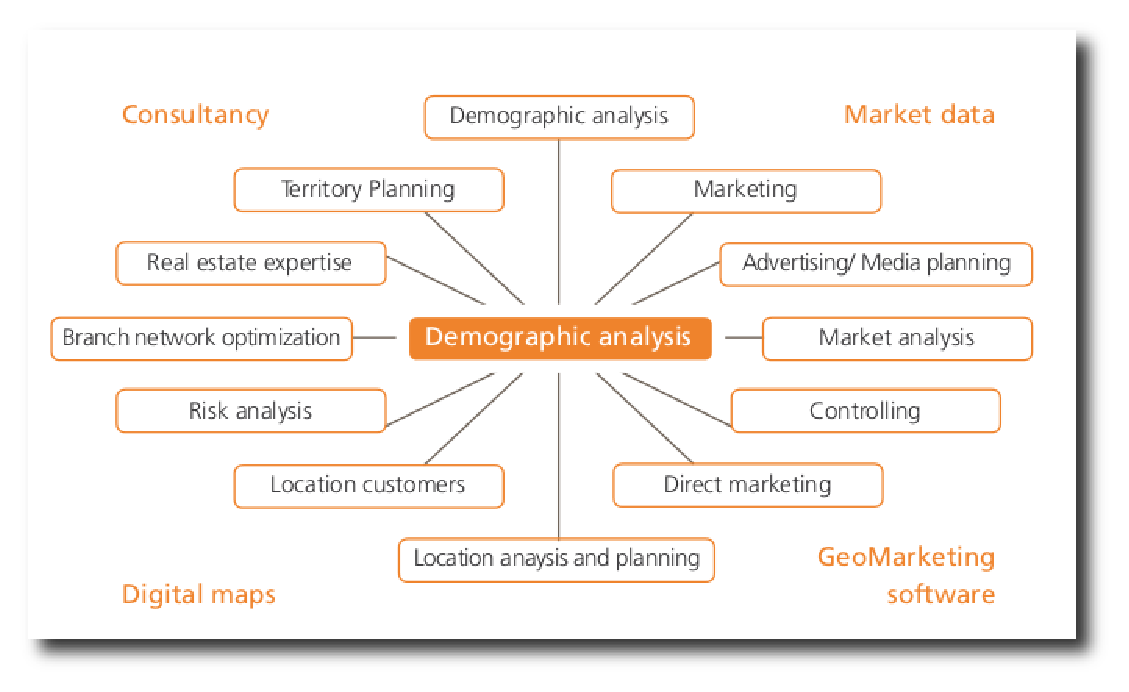
\includegraphics[scale=0.8]{Figures/Geomarketing_application.eps}
  \end{center}
  \caption{Some Geomarketing applications}
  \label{Some Geomarketing applications}
\end{figure}

\section{Software solution}
A crucial component of geomarketing is the visualization of data via a
specialized geomarketing software application. Working with this software
involves several straightforward steps:

\begin{itemize}
  \item Selecting appropriate maps
  \item Importing data
  \item Data evaluation
  \item Exporting result
\end{itemize}